\documentclass[aspectratio=43]{beamer}
\usepackage[english]{babel}
\usepackage{amsthm}
\usepackage{mathtools}
\usepackage{physics}
\usepackage{calligra}
\usepackage{csquotes}
\usepackage{tensor}
\usepackage[thicklines]{cancel}
\usepackage{tcolorbox}
\usepackage{pstricks}
\usepackage[backend=biber, bibstyle=nature, sorting=nty, citestyle=numeric-comp]{biblatex} %Custom bibliography
    \addbibresource{bib.bib} %Load references


\DeclareMathAlphabet{\mathcalligra}{T1}{calligra}{m}{n}
\DeclareFontShape{T1}{calligra}{m}{n}{<->s*[2.2]callig15}{}
\newcommand{\scriptr}{\mathcalligra{r}\,}
\newcommand{\boldscriptr}{\pmb{\mathcalligra{r}}\,}
\def\rc{\scriptr}
\def\brc{\boldscriptr}
\def\hrc{\hat\brc}
\newcommand{\ie}{\emph{i.e.}} %id est
\newcommand{\eg}{\emph{e.g.}} %exempli gratia
\newcommand{\rtd}[1]{\ensuremath{\left\lfloor #1 \right\rfloor}}
\newcommand{\dirac}[1]{\ensuremath{\delta \left( #1 \right)}}
\newcommand{\diract}[1]{\ensuremath{\delta^3 \left( #1 \right)}}
\newcommand{\e}{\ensuremath{\epsilon_0}}
\newcommand{\m}{\ensuremath{\mu_0}}
\newcommand{\V}{\ensuremath{\mathcal{V}}}
\newcommand{\prnt}[1]{\ensuremath{\left(#1\right)}} %parentheses
\newcommand{\colch}[1]{\ensuremath{\left[#1\right]}} %square brackets
\newcommand{\chave}[1]{\ensuremath{\left\{#1\right\}}}  %curly brackets

\useoutertheme{infolines}
\useinnertheme{rectangles}
\usefonttheme{professionalfonts}


\definecolor{rose}{HTML}{e63c73}
\definecolor{gray}{HTML}{303030}
\definecolor{yellow}{HTML}{f0be52}
\definecolor{lightrose}{HTML}{fe73a0}

\renewcommand{\CancelColor}{\color{rose}}

\makeatletter
\newcommand{\mybox}[1]{%
  \setbox0=\hbox{#1}%
  \setlength{\@tempdima}{\dimexpr\wd0+13pt}%
  \begin{tcolorbox}[colback=rose,colframe=rose,boxrule=0.5pt,arc=4pt,
      left=6pt,right=6pt,top=6pt,bottom=6pt,boxsep=0pt,width=\@tempdima]
    \textcolor{white}{#1}
  \end{tcolorbox}
}
\makeatother

\usecolortheme[named=rose]{structure}
\usecolortheme{sidebartab}
\usecolortheme{orchid}
\usecolortheme{whale}
\setbeamercolor{alerted text}{fg=lightrose}
\setbeamercolor{block title alerted}{bg=alerted text.fg!90!black}
\setbeamercolor{block title example}{bg=lightrose!60!black}
\setbeamercolor{background canvas}{bg=gray}
\setbeamercolor{normal text}{bg=gray,fg=white}

\setbeamertemplate{footline}
        {
      \leavevmode%
      \hbox{%
      \begin{beamercolorbox}[wd=.333333\paperwidth,ht=2.25ex,dp=1ex,center]{author in head/foot}%
        \usebeamerfont{author in head/foot}\insertshortauthor~~(\insertshortinstitute)
      \end{beamercolorbox}%
      \begin{beamercolorbox}[wd=.333333\paperwidth,ht=2.25ex,dp=1ex,center]{title in head/foot}%
        \usebeamerfont{title in head/foot}\insertshorttitle
      \end{beamercolorbox}%
      \begin{beamercolorbox}[wd=.333333\paperwidth,ht=2.25ex,dp=1ex,center]{date in head/foot}%
        \usebeamerfont{date in head/foot}\insertshortdate{}%\hspace*{2em}

    %#turning the next line into a comment, erases the frame numbers
        %\insertframenumber{} / \inserttotalframenumber\hspace*{2ex} 

      \end{beamercolorbox}}%
      \vskip0pt%
    }


\setbeamertemplate{blocks}[rectangle]
\setbeamercovered{dynamic}

\setbeamertemplate{section page}
{
	\begin{centering}
		\begin{beamercolorbox}[sep=27pt,center]{part title}
			\usebeamerfont{section title}\insertsection\par
			\usebeamerfont{subsection title}\insertsubsection\par
		\end{beamercolorbox}
	\end{centering}
}

%\setbeamertemplate{subsection page}
%{
%	\begin{centering}
%		\begin{beamercolorbox}[sep=12pt,center]{part title}
%			\usebeamerfont{subsection title}\insertsubsection\par
%		\end{beamercolorbox}
%	\end{centering}
%}

\newcommand{\hlight}[1]{\colorbox{violet!50}{#1}}
\newcommand{\hlighta}[1]{\colorbox{red!50}{#1}}
\title{Shake-Eat} %->->->->-> Check hyperref title <-<-<-<-<-
\subtitle{L'application qui choisit pour vous}
\author[Emilie LEBON et Matthias BERJOLA]{Emilie LEBON et Matthias BERJOLA}
\begin{document}
\centering 
\includegraphics[height = 0.25 \textheight]{images/ufr-st.png}
\centering 
\includegraphics[height =0.25 \textheight]{images/logo_universite.jpg}
\institute[LIM]{
    LIM%
    \\%
    Université de la Réunion%
} %You can change the Institution if you are from somewhere else
\date{Novembre 2020}
%\logo{\includegraphics[width= 0.2\textwidth]{images/a-logo.png}}


    
    \frame{\titlepage}
    
    \begin{frame}{Sommaire}
        \tableofcontents
    \end{frame}
    
    \input{chapters/Présentation} %You can put the frames directly into the presentation, but using the input command and writing them in separate .tex files might be more organized
    
    \section{Fonctionnalités} 


    
    \frame{\sectionpage}
    
   
    \begin{frame}{Géolocalisation}
        \centering
        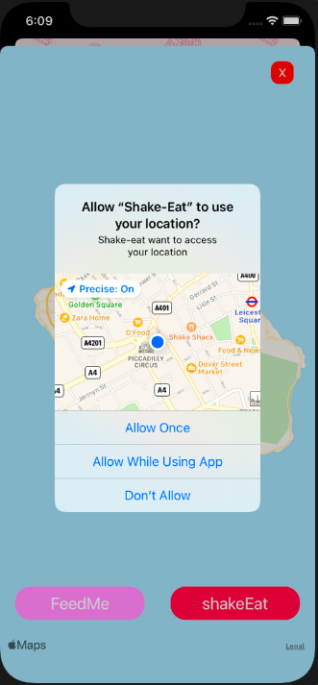
\includegraphics[height = 0.8 \textheight]{images/geoloc.png}
        
    \end{frame}
    
     \begin{frame}{La carte : Affichage des restaurants du coin}
        \centering
        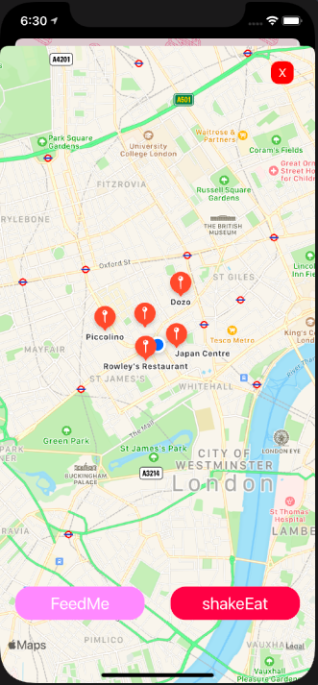
\includegraphics[width = 0.25\textwidth]{images/carte-tous-restos.png}
    \end{frame}
    
    \begin{frame}{Code Intéressant : choix aléatoire d'un point}
        \centering
            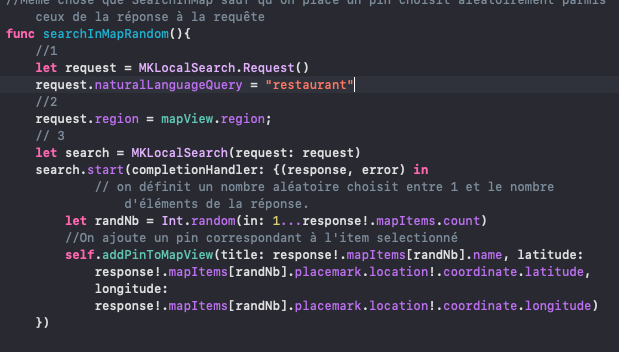
\includegraphics[height = 0.6 \textheight]{images/code-aleatoire.png}
    \end{frame}
    
    
    \begin{frame}{Pop-Up}
        La Pop-Up demande à l'utilisateur de secouer son téléphone
        \centering
        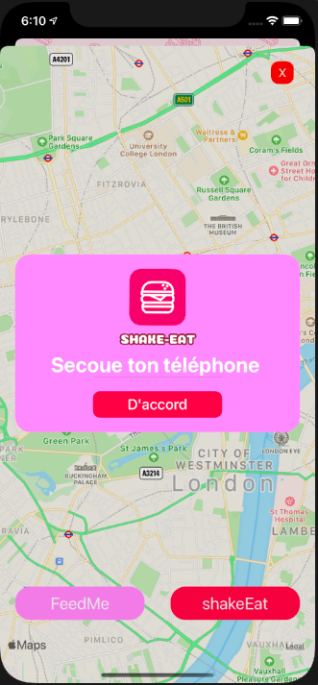
\includegraphics[width = 0.25\textwidth]{images/carte-post-shake.png}
    \end{frame}
    
    
    
    
    
    
    
    
    \section{Améliorations possibles}

\section{Conclusion}

    \subsection{}
    \frame{\sectionpage}

    
    
    \begin{frame}{Conclusion}
        \begin{block}{\centering Nous vous remercions de votre attention !}
             \centering \alert{ BERJOLA Matthias et LEBON Emilie}
        \end{block}
    \end{frame}
    
    
    \begin{frame}{Shake your choice, Shake-Eat !}
        \centering
        Si vous ne savez pas où manger, laissez Shake-Eat choisir pour vous !
    \end{frame}
    
    \section*{Remerciements} %You can remove this if you do not want to use it
        \begin{frame}{Remerciements}
        \begin{center}
            
       
            Je tiens à remercier David Blain, qui a posé la question qui nous a permis de nous décider pour notre application : \\ "Qu'est-ce qu'on mange ce midi ?"
        \end{center}
        \end{frame}
    
   

    \section{}
    \begin{frame}{}
        \centering
            \Huge\bfseries
        \textcolor{rose}{The End}
    \end{frame}
\end{document}
